% Typical moment-rotation curves of beam-to-column connections (after Chen & Toma 1994, Fig. 1.8)
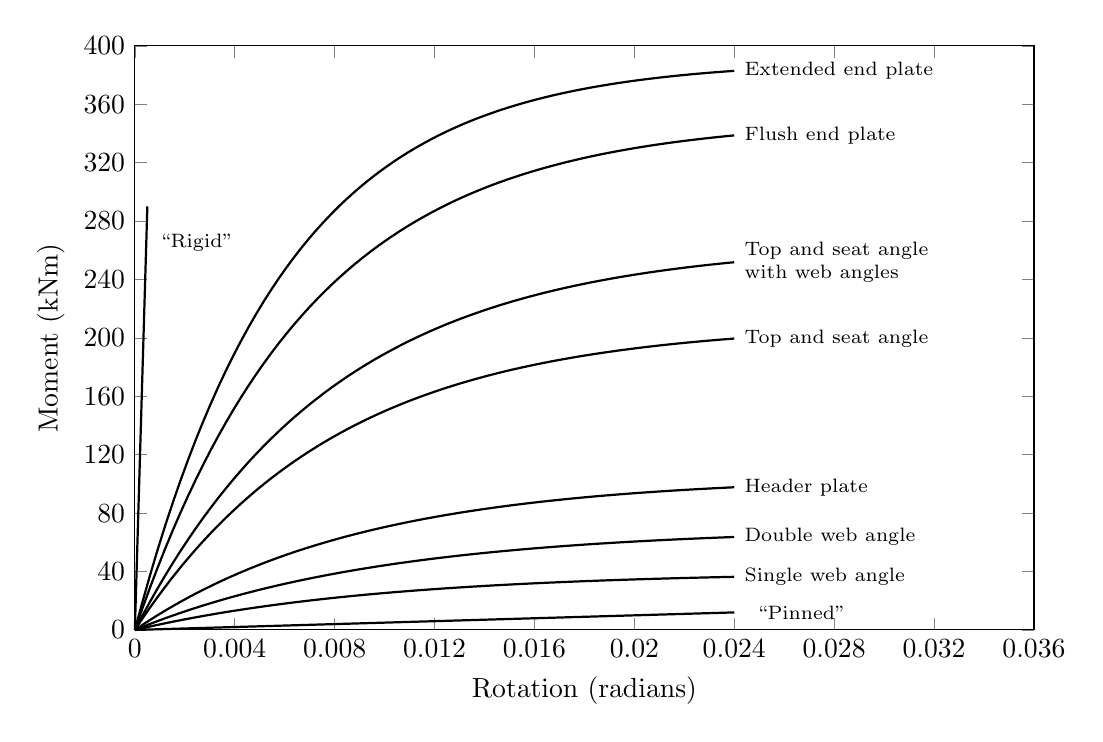
\begin{tikzpicture}
  \begin{axis}[
    width=13cm,height=9cm,
    xlabel={Rotation (radians)},ylabel={Moment (kNm)},
    xmin=0,xmax=0.036,ymin=0,ymax=400,
    xtick={0,0.004,...,0.036},xticklabel style={/pgf/number format/fixed,/pgf/number format/precision=3},
    ytick={0,40,...,400},
    clip=false,samples=80,domain=0:0.024,
    every axis plot/.append style={thick,black},
    cycle list={{black},{black},{black},{black},{black},{black},{black}},
    scaled x ticks=false,
  ]
    % curves of the form M = M0 * (1 - exp(-x/c))
    \addplot {390*(1-exp(-x/0.006))} node[right,font=\scriptsize] {Extended end plate};
    \addplot {350*(1-exp(-x/0.007))} node[right,font=\scriptsize] {Flush end plate};
    \addplot {265*(1-exp(-x/0.008))} node[right,align=left,font=\scriptsize] {Top and seat angle\\with web angles};
    \addplot {210*(1-exp(-x/0.008))} node[right,font=\scriptsize] {Top and seat angle};
    \addplot {105*(1-exp(-x/0.009))} node[right,font=\scriptsize] {Header plate};
    \addplot {70*(1-exp(-x/0.010))} node[right,font=\scriptsize] {Double web angle};
    \addplot {40*(1-exp(-x/0.010))} node[right,font=\scriptsize] {Single web angle};
    \draw[thick] (axis cs:0,0) -- (axis cs:0.0005,290); \node[right,font=\scriptsize] at (axis cs:0.0006,265) {``Rigid''};
    \draw[thick] (axis cs:0,0) -- (axis cs:0.024,12); \node[right,font=\scriptsize] at (axis cs:0.0245,12) {``Pinned''};
  \end{axis}
\end{tikzpicture}
